\begin{figure}[H]
\centering
\def\axislength{.2}
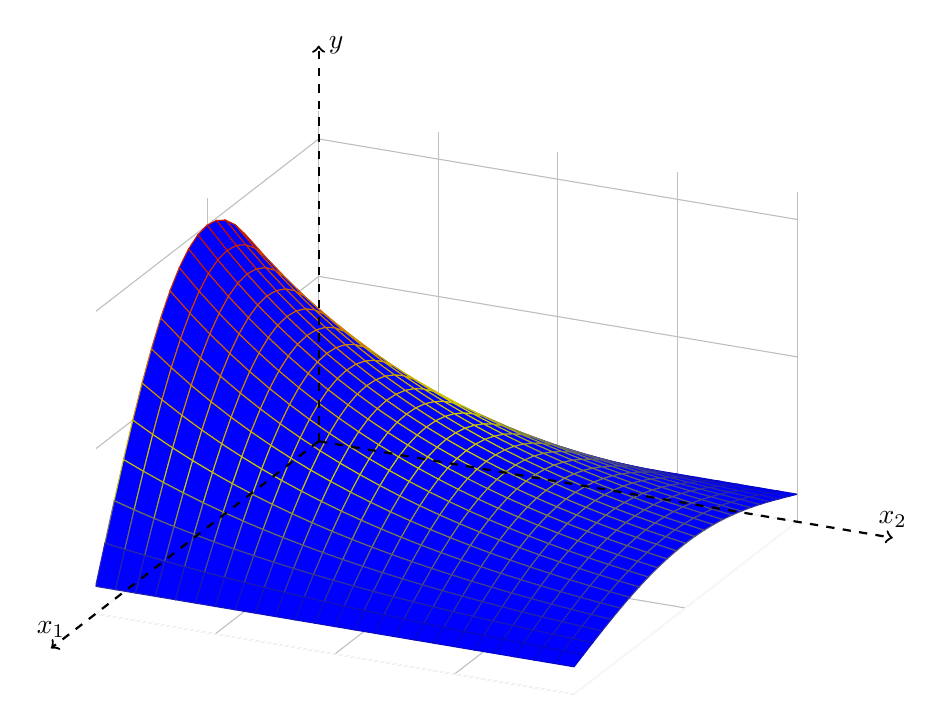
\begin{tikzpicture}
\pgfplotsset{
    axis line style={white},
  }
  \begin{axis}[scale=1.3,ticks=none, grid=major, legend style={at={(1.1,1.1)},anchor=north west} ]
    \coordinate (O) at (rel axis cs:0,1,0);
    \coordinate (x) at (rel axis cs:0,-\axislength,0);
    \coordinate (y) at (rel axis cs:1+\axislength,1,0);
    \coordinate (z) at (rel axis cs:0,1,1+\axislength);
    \addplot3[surf,shader=faceted,
			samples=25,domain=0:2,y domain=0:1, color=blue] {exp(-x) * sin(pi*deg(y))};
  \end{axis}
  \draw[thick,dashed,->] (O) -- (x) node[above] {$\boldsymbol{x_1}$};
  \draw[thick,dashed,->] (O) -- (y) node[above] {$\boldsymbol{x_2}$};
  \draw[thick,dashed,->] (O) -- (z) node[right] {$\boldsymbol{y}$};

  
\end{tikzpicture}
\caption[Erste Vorstellung der Funktion in Bezug auf die Koordinaten des Schusses]{Erste Vorstellung der Funktion in Bezug auf die Koordinaten des Schusses\protect\footnotemark}
\label{vermutung}
\end{figure}
\footnotetext{Eigene Darstellung}